
\subsection{Überblick über den Umrichter-Prüfstand}
\label{subsec:uberblick-uber-den-umrichter-prufstand}

In diesem Abschnitt wird der Umrichter-Teststand, von dem die zu verarbeitenden Datensätze stammen, beschrieben,
da dies für das generelle Verständnis der einzulesenden Datensatzstruktur unerlässlich ist.
Die genaue Bezeichnung des Teststandes „USTB DWT Test Bench (XCT0006-1)“ wird im Folgenden als Test-Bench oder Teststand benannt.
Diese Art Test-Bench wird im Allgemeinen für die End-of-Line-Prüfung von unterschiedlichen Umrichtern nach ihrer Herstellung genutzt,
um die Produktqualität und -funktionalität sicherzustellen. \cite*{Main_Manuel_USTB2018}

In dem hier vorliegenden Fall wird der Teststand verwendet, um die aus dem Feld kommenden Umrichter auf ihre weitere Nutzungstauglichkeit zu testen.
Die weitere Nutzungstauglichkeit wird ermittelt, indem die Messwerte mit Mittelwerten, die von mehreren fabrikneuen Umrichtern stammen, verglichen werden.
Diese Messwerte müssen sich in einem vorher definierten Toleranzbereich befinden, um weiter im Feld verwendet zu werden.

Die Umrichter werden in der gegebenen Fachliteratur zur Test-Bench als \ac{DUTs} bezeichnet.
Diese Bezeichnung kommt auch in den Berichten auf dem Teststand vor, daher hat der Autor diese Abkürzung übernommen.

%------------------------------------------------------------------------------------------------------
\subsubsection{Aufbau des Teststandes}
%------------------------------------------------------------------------------------------------------
Die Test-Bench besteht aus mehreren Komponenten, die sich im Testraum in unterschiedlichen Schaltschränken befinden.
Der Teststand besteht aus folgenden Hauptkomponenten:
Die Test-Bench besteht aus mehreren Komponenten, die sich im Testraum in unterschiedlichen Schaltschränken befinden, und der Teststand umfasst folgende Hauptkomponenten:
\begin{itemize}

\item Das Netzteil wandelt die 400-V-Netzspannung in eine isolierte Gleichspannung für den Zwischenkreis um.
Das Netzteil liefert maximal 80 kW mit 1200 V DC oder 800 V DC, welche Werte verwendet werden, kann vor Teststart bestimmt werden.
In Abbildung \ref{fig: Aufbau des Teststandes} wird das Netzteil als PSU bezeichnet, was für „Power Supply Unit“ steht.
\item Das Elektronik-Rack, auf dem die Mess- und Steuerkomponenten befestigt sind, ist ein wichtiger Bestandteil des Teststandes.
Hier befindet sich auch der (XCS2100) System-Controller, der das ganze System mit dem PC, auf dem die Test-Bench-Software läuft, via Ethernet verbindet.
In Abbildung \ref{fig: Aufbau des Teststandes} mit ER bezeichnet, für „Electronic Rack“.
\item Der Testmatrix-Schrank, in dem die Sammelschienen für den Stromanschluss und die Schützen sitzen.
In Abbildung \ref{fig: Aufbau des Teststandes} mit TM bezeichnet, für „Test Matrix cabine“.
\item Der Schrank mit dem Kühlungssystem, da die Umrichter während des Betriebes mit Wasser oder Luft gekühlt werden müssen.
In Abbildung \ref{fig: Aufbau des Teststandes} mit „Cool1“ bezeichnet.
\item Der Carrier, auf dem die Umrichter befestigt werden, ist speziell für bestimmte Umrichter konstruiert.
Dieser wird speziell für bestimmte Umrichter konstruiert.
In Abbildung \ref{fig: Aufbau des Teststandes} wird der Carrier als Carrier1 bezeichnet.

\end{itemize}

Neben den Hauptkomponenten befinden sich außerhalb des Sicherheitsbereiches, der während des Betriebes nicht betreten werden darf,
ein PC mit einer Software zum Steuern der Testeinrichtung sowie eine Betriebsanzeige und ein Notaus. \cite*{Main_Manuel_USTB2018}

\begin{figure}[h]
    \centering
    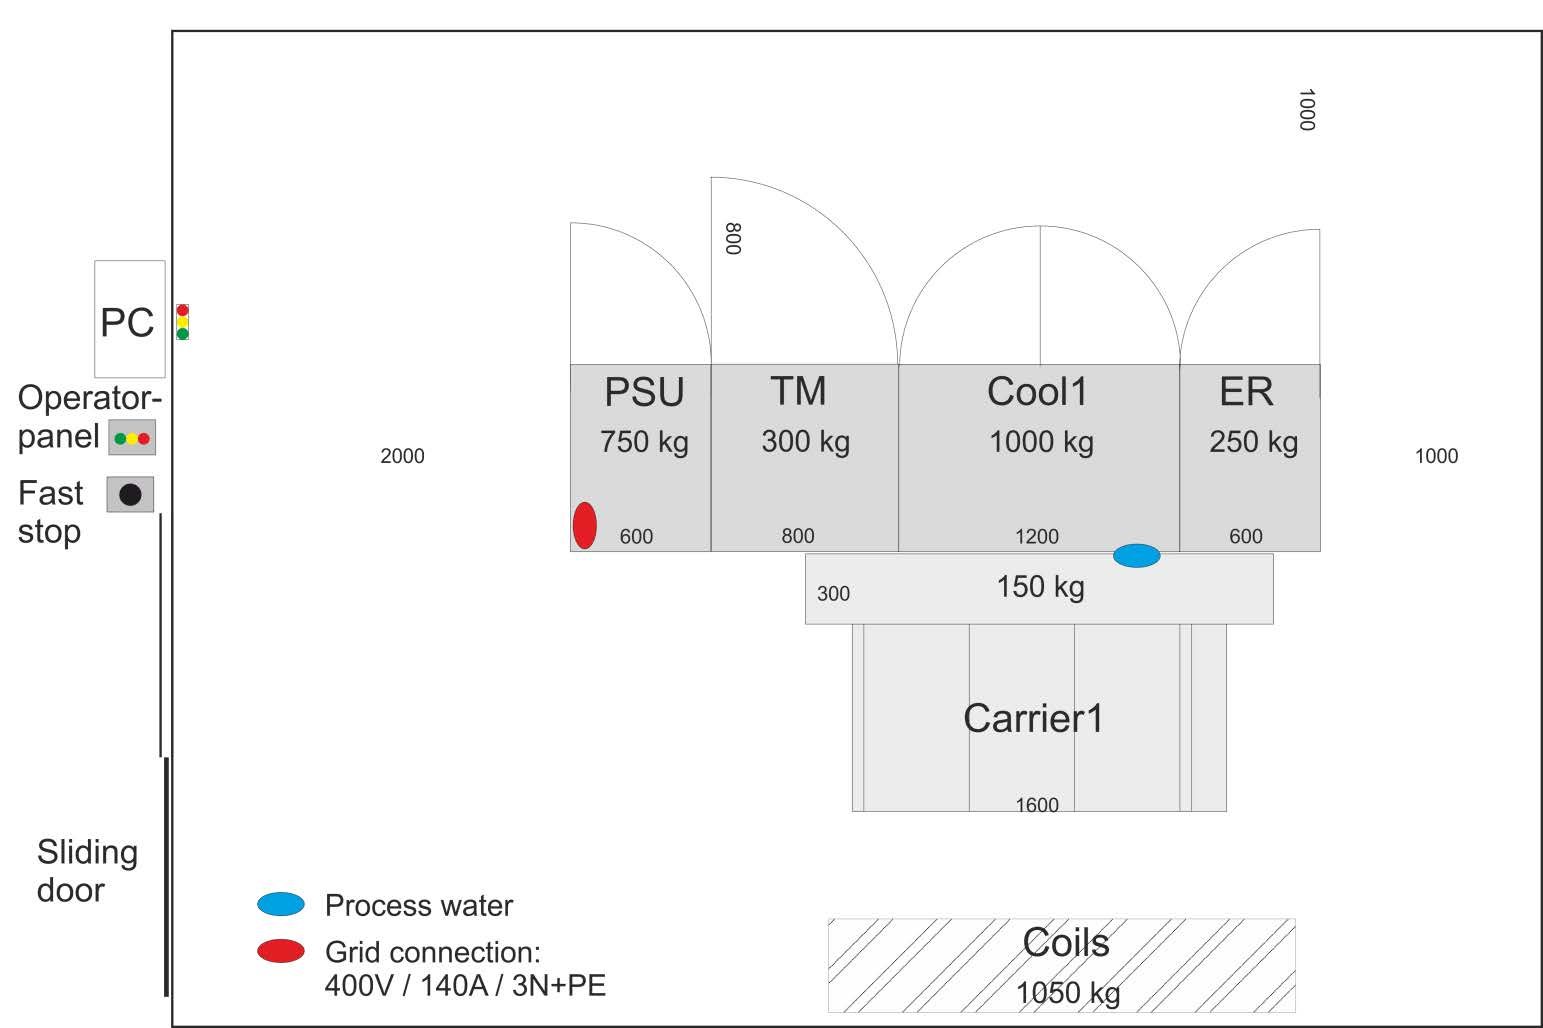
\includegraphics[width=0.8\textwidth]{Grafiken/Test Cabin}
    \caption{Aufbau des Teststandes}
    \label{fig: Aufbau des Teststandes}
    {Quelle: \cite*[7]{Main_Manuel_USTB2018}}
\end{figure}
%------------------------------------------------------------------------------------------------------
\subsubsection{Testmodule}
%------------------------------------------------------------------------------------------------------
Es gibt mehrere Testmodule, die auf dem Teststand laufen und verschiedene Funktionen der Umrichter testen.
Einige der Funktionen eines DUT können mit dem gleichen Modus eines Testmoduls überprüft werden, indem die entsprechenden Parameter ausgewählt werden.
Jeder Testablauf ist autonom und kann mehrmals ausgeführt werden, auch mit unterschiedlichen Parametern.
\\
Im Folgenden wird eine kurze Beschreibung der Funktionen der für diese Arbeit relevanten Testmodule gegeben.

Driver Consumption Test:
Der Driver Consumption Test überprüft den Stromverbrauch des Treibers im Leerlauf und während Pulssprüngen.

Pulse Test:
Der Impulstest verfügt über drei Funktionsmodi.
\begin{itemize}
    \item Im Modus \ac{FSW} kann überprüft werden, ob die Halbleiter, die sich in den \ac{DUTs} befinden, generell schalten.
    \item Im Modus \ac{OCP} kann die Überstromüberwachung weiche Kurzschlüsse überprüfen.
    Ein weicher Kurzschluss ist, wenn der Stromfluss nicht sofort und vollkommen unterbrochen wird.
    \item Im Modus \ac{DSCP} wird ein harter Kurzschluss, also ein vollständiger und sofortiger Kurzschluss, überprüft.
\end{itemize}


Power Test:
Mit diesem Test werden zwei verschiedene Funktionen getestet werden:

\begin{itemize}

    \item \ac{BIT} dient dazu, die \ac{DUTs} zyklisch zu betreiben und so reale Betriebszustände zu simulieren.
    Zudem kann mit Hilfe dieser Funktion die Kühltemperatur überprüft werden, um die korrekte Wärmeübertragung der Halbleiter sicherzustellen.
    \item Während des \ac{OTP} wird ein DUT, ähnlich wie beim \ac{BIT}, nur mit reduzierter
    Kühlung betrieben, bis die maximal zulässige Kühlkörpertemperatur erreicht ist und die Temperaturschutzschaltung auslöst.\cite*{Main_Manuel_USTB2018}

\end{itemize}

%------------------------------------------------------------------------------------------------------
\subsubsection{Testablauf}
%------------------------------------------------------------------------------------------------------
Die Schrittfolge des Testablaufes mit Montage der \ac{DUTs} ist klar festgelegt und vor jedem Durchlauf gleich.
Die Montage läuft wie folgt ab:
\begin{enumerate}

\item Die Umrichter werden auf dem Carrier befestigt. Es werden meist 3 dieser Geräte gleichzeitig getestet, Abweichungen je nach Bauform.
Die Reihenfolge der elektrischen Phasen ist bei Draufsicht des Carriers von links nach rechts U-V-W. Dies ist für das Layout des Berichtes relevant.
\item Der Kühlkreislauf wird angeschlossen, je nach Umrichtertyp Lüftungs- oder Wasserkühlung.
\item Die \ac{DUTs} werden mit den AC- und DC-Link-Kontakten verbunden, um das Gerät zu betreiben und die DC-Spannung wieder abzuleiten.
\item Das Anbringen von Signalkabeln zwischen DUT und Merkurbox. Die Merkurbox dient als Schnittstelle zwischen \ac{DUTs} und Testbench.
\item Das Montieren von VCE-Klemmen an die AC-Kontakte der \ac{DUTs}.

\end{enumerate}

Vor Beginn des Testablaufs benötigt die Test-Bench noch weitere Informationen zu den \ac{DUTs}, Testsequenzen und der Hardware-Topologie.
Diese Daten können über das Scannen von vorliegenden QR- oder Barcodes eingefügt werden.
Alternativ können diese auch über ein Eingabefenster im Teststandprogramm eingetragen werden.
Je nach Topologiekonfiguration kann auch ein zweiter Träger mit \ac{DUTs} gescannt werden,
Dies kommt bei dem Test, den das Unternehmen durchführt, nicht vor. \cite*{Main_Manuel_USTB2018}

Das eigentliche Testen mit den verschiedenen Testmodulen wird autonom durchgeführt.
Im Unternehmen läuft der Test regulär wie folgt ab:
\begin{enumerate}

\item Durchführung des Driver Consumption Testes, um die Stromversorgung der Treiberplatine auf den Umrichter zu testen.
\item Durchführung des Pulse Testes im Modus Functional-Switching, dies prüft die Umrichter.
\item Durchführung des Power Testes, in den Berichten auch XPower Test genannt.
Dieser Test simuliert die Belastung der Umrichter im Feld und überprüft,
ob sich die Werte in einem bestimmten Toleranzbereich befinden.

\end{enumerate}

Nach dem Durchlaufen eines Tests wird automatisch ein \ac{XML}-Datenfile mit den erhobenen Messdaten generiert,
die enthaltenen Messwerte und alle vorher bestimmten Einstellungen erstellt und in eine Datei eingefügt.

Bei der Demontage nach dem Testdurchlauf werden alle Schritte in umgekehrter Reihenfolge durchgeführt.
%------------------------------------------------------------------------------------------------------
\pagebreak



